In this Section, we study the information that we can infer from the dataset about the battles and how they evolved in history. We start by observing how the duration of the battles and the number of casualties progressed during a millennium. Then, we interest ourselves in the outcome of the battles, we try to determine on what depends a victory for a combatant and how we can predict or not the result of a conflict. 
\subsection{Duration of the Battles}

We observe that the duration of the battles over the last millenium almost continually increased. In fact, in Figure \ref{fig:durThByCent}, we observe that the order of magnitude of the duration of a battle has never been higher than nowadays. The average duration of a battle was almost 34 days during the XX$^{th}$ century and is currently of 64 days in the XXI$^{st}$ century.

 \begin{figure}[h]
	\centering	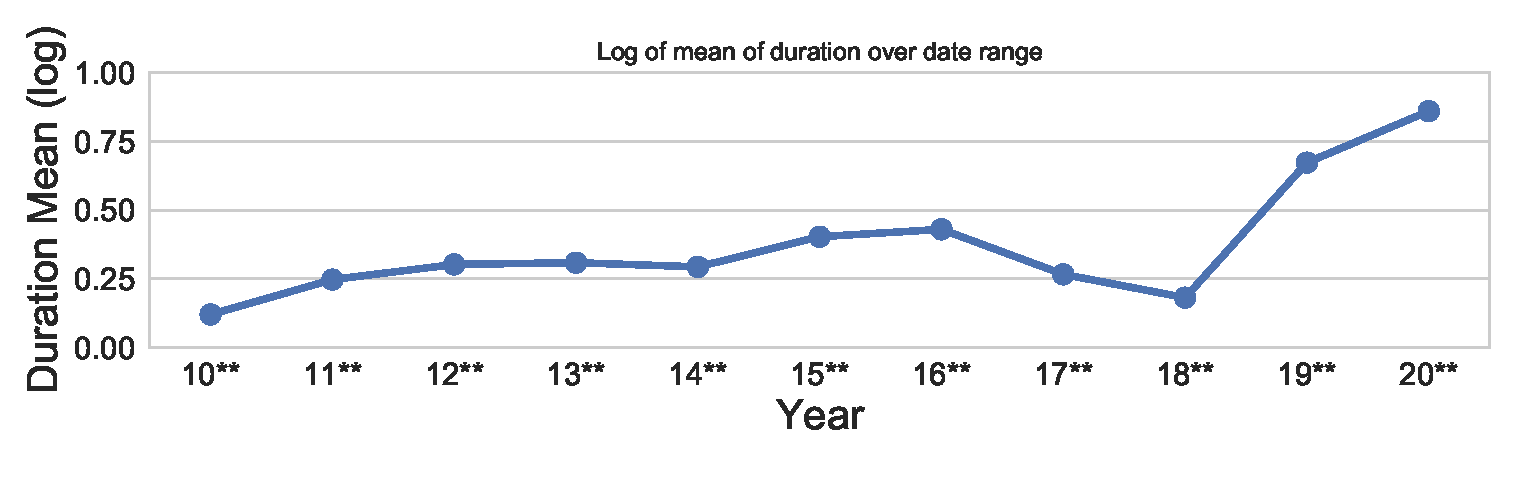
\includegraphics[width=\linewidth]{figures/durThByCent}
	\caption{Mean of the duration of battles in the last thousand years by century on a logarithmic scale.}\label{fig:durThByCent}
	\centering
\end{figure}

\subsection{Evolution of the Casualties}

In Figure \ref{fig:casuPerCent}, we notice that the percentage of soldiers engaged in a battle that are wounded, killed, captured or that disappeared decreases among the years. We observe that, as it is the case in Figure \ref{fig:durThByCent} for the battle's duration, the percentage of casualties decreased before increasing in the XX$^{th}$ century. We can infer that in both cases this is due to the world wars that both contain numerous battles which made countless casualties, notably because of technology advances such as aerial forces or gaz attacks.
 \begin{figure}[h]
	\centering	\includegraphics[width=\linewidth]{figures/casuPerCent}
	\caption{Mean of the percentage of casualties in the soldiers.}\label{fig:casuPerCent}
	\centering
\end{figure}

\subsection{Indecisiveness of the Battles}

We observe, in Figure \ref{fig:IndecBattles}, that battles are more indecisive nowadays than they were in the past. In fact, this number (in order of magnitude) is increasing since year 1200 and shows an higher increase for the last last century and now. This can be explained by two factors: battles in the further past were probably often reported by the winner which wouldn't consider it as indecisive and again the two world wars in the  XX$^{th}$ century also contain a lot of strategic and indecisive battles that served a higher or more general goal.
 \begin{figure}[h]
	\centering	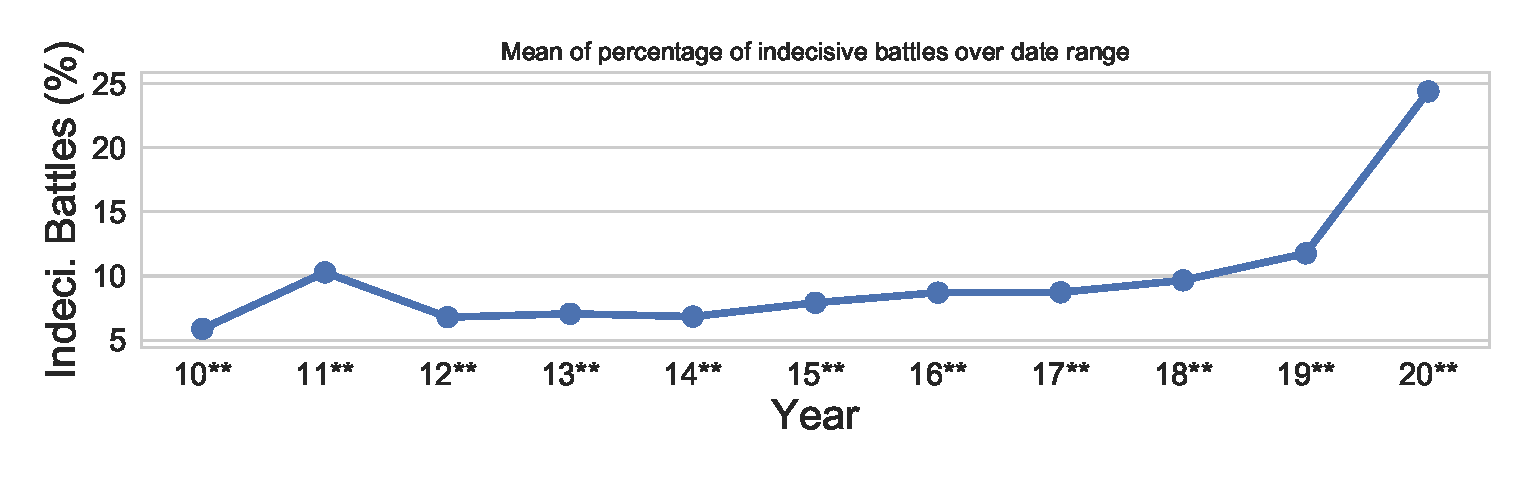
\includegraphics[width=\linewidth]{figures/indThByCent}
	\caption{Mean of the number of indecisive battles over the last thousand years by century on a logarithmic scale.}\label{fig:IndecBattles}
	\centering
\end{figure}

From Figures \ref{fig:durThByCent}, \ref{fig:casuPerCent} and \ref{fig:IndecBattles}, we conclude that battles became longer, made less casualties and were more indecisive over the years. This supports the fact that nowadays the battles purpose is not only to invade another territory by beating the other combatant. In fact, modern battles seems to be more complicated in the sense that they often serve a higher strategic goal and do not always results in a decisive victory.

\subsection{Outcome of the Battles}

With Figure \ref{fig:victoryAdvantage}, we study the importance for a combatant to have an advantage in the number of casualties (less victims), the number of soldiers (higher strength) and the percentage of casualties among soldiers. We show the percentage of battles that were won and resulted in a decisive, strategic, tactical or any victory for a combatant that had an advantage in one of these features. Our main observation is that the combatant that had less casualties won in almost 80\% of the cases. A higher strength resulted in a victory in less than 50\% of the battles, which means that if we wanted to predict the winner of a battle, we should simply choose the combatant that suffers less casualties. In order to support our hypothesis, we trained a random forrest classifier on our dataset and it also simply chose the number of casualties to decide for the winner of a battle.

We notice that the number of casualties is less important for a strategic victory when the goal is not to inflict more damages to the opponent but to progress for a more general purpose.
 \begin{figure}[h]
	\centering	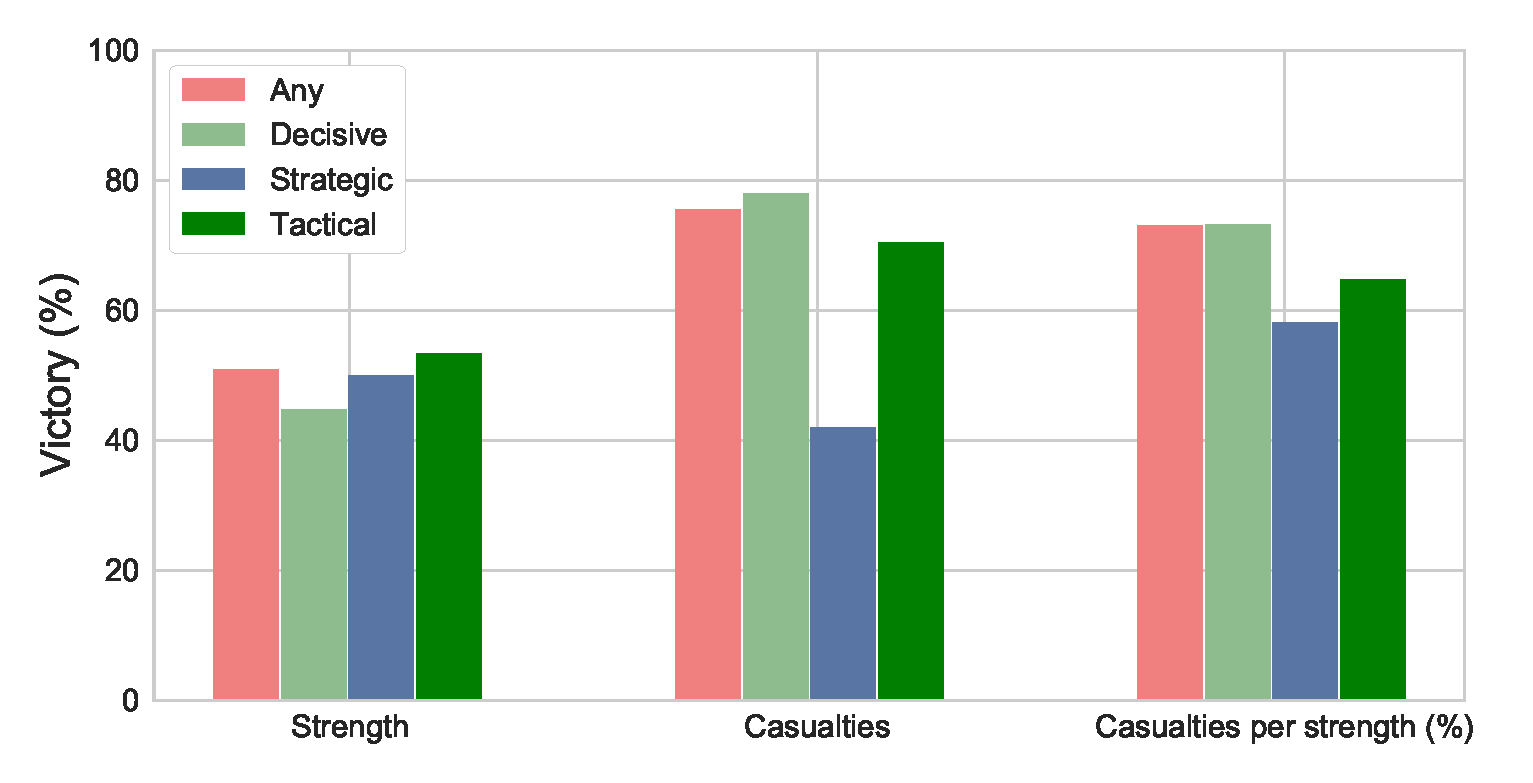
\includegraphics[width=\linewidth]{figures/VictoryAdvantage}
	\caption{Victory percentage when advantage in either strength, casualties or percent of casualties in the strength.}\label{fig:victoryAdvantage}
	\centering
\end{figure}

\subsection{Years of Battles per Countries}
In Figure \ref{fig:FightingDurationRanking}, we observe that among all the countries, France is the one that fought the most. Nevertheless, the United States, which are a major actor in the international history of battles, were only created in 1776 when they proclaimed their independence. Thus, it is interesting to do the same ranking starting from this year. 
 \begin{figure}[h]
	\subfigure[]{\includegraphics*[width=0.5\linewidth]{figures/YearsFightingRanking}} 
	\hspace{-0.4 em}
	\subfigure[]{\includegraphics*[width=0.5\linewidth]{figures/YearsFightingRankingModern}}
	\vspace{-0.1 em}
	\caption{Cumulated duration of battles engagement per country. From 100 in (a) and from 1776 and the United States independence in (b).} 
	\label{fig:FightingDurationRanking}
\end{figure}
 These results tend to support the common belief that the United States are always in war. In fact, as we observe in Figure \ref{fig:USAFightingTimeline}, they were engaged in a at least one battle per year for more than 150 years in 242 years of existence.
 \begin{figure}[h]
 	\centering	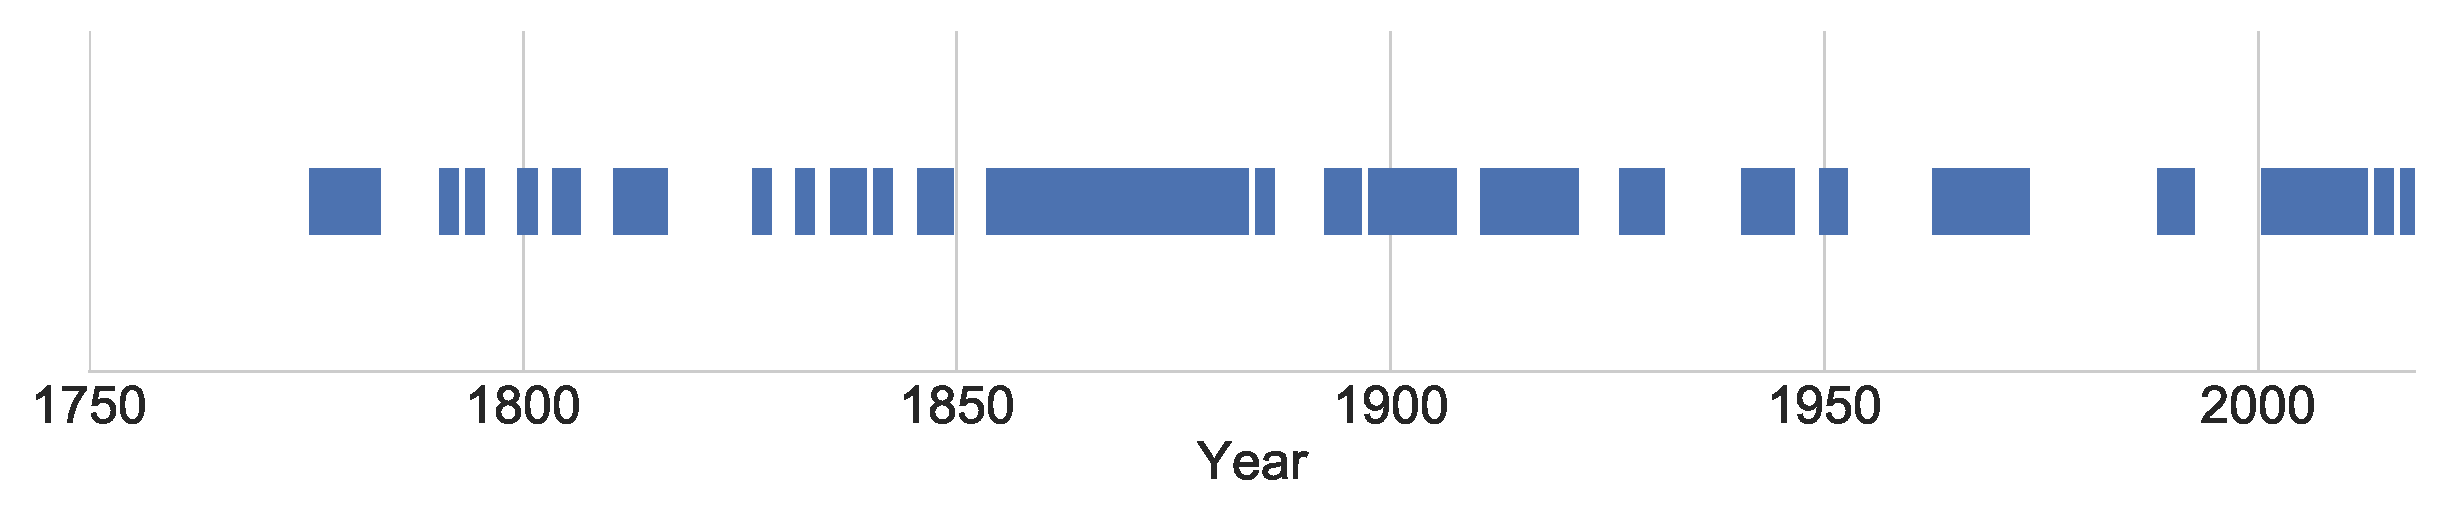
\includegraphics[width=\linewidth]{figures/USAFighting}
 	\caption{Timeline of the USA engagement in battles.}\label{fig:USAFightingTimeline}
 	\centering
 \end{figure}

